\subsection{Rotation Measurement}\label{ssec:speedMeasurement}
	
	As it was specified in Item \ref{itm:monitored-speed} from Section \ref{ssec:monitored-parameters}, monitoring the rotor speed is mandatory in order to perform brake tests. There are many different ways to measure speed in rotors and shafts. On the automotive environment this measurements are done using magnetic sensors.
	\par
	The name used for the sensor in the automotive environment is Crankshaft Position Sensor (CKP), it has this name because most of the time this sensor is mounted aligned with the crankshaft and is used to monitor both the speed and the position of the crankshaft. A typical CKP sensor is shown in Figure \ref{fig-ckpReal}.

	\begin{figure}[htbp]
		\centering
		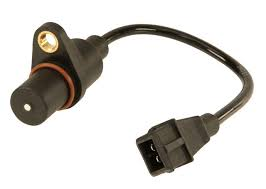
\includegraphics[width=.5\textwidth]{figuras/fig-ckp-real.jpg}
		\caption{\textit{Crankshaft Position Sensor} \cite{ckp-gm}}
		\label{fig-ckpReal}
	\end{figure}

	This sensor is widely used in the automotive industry to determine the angular position of the vehicle's crankshaft and its rotation speed. There are several types of CKP sensors, the most common are the variable reluctance type because they have low cost and good accuracy \cite{schroeder2002crankshaft}.
	\par
	As the gear in question rotates each tooth of the gear aligns with the variable reluctance sensor, a magnetic flux in the sensor coil changes as the air gap between the sensor and the gear changes. This change in the magnetic field generates induces a voltage pulse at the sensor output. This type of sensors have an analog voltage output where amplitude and frequency vary proportionally to the speed of rotation of a gear, as Figure \ref{fig:ckp-signal}. With this type of sensor it is possible to extract data of linear velocity, angular velocity and angular position. However, only the angular velocity data (frequency) is important to be measured for brake tests specified by the regulation \cite{saej2522}. 

	\begin{figure}[htbp]
		\centering
		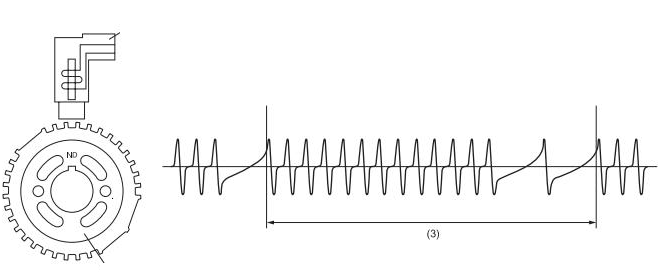
\includegraphics[width=.8\textwidth]{figuras/fig-ckp-signal.png}
		\caption{Magnetic Sensor Signal \cite{cam-sensor-signal}}
		\label{fig:ckp-signal}
	\end{figure}